%!TeX program = xelatex
\documentclass[12pt,hyperref,a4paper,UTF8,fontset=fandol]{ctexart}
\usepackage{SDUReport}
\usepackage{booktabs}
\usepackage{amsmath}
\usepackage{float}
\usepackage{graphicx}

%%-------------------------------正文开始---------------------------%%
\begin{document}

%%-----------------------封面--------------------%%
\cover

\thispagestyle{empty}

%%--------------------------目录页------------------------%%
\newpage
\pagenumbering{Roman}
\tableofcontents

%%------------------------正文页从这里开始-------------------%
\newpage
\pagenumbering{arabic}

\section{项目背景与任务描述}

本实验围绕轮胎点云展开后的轮廓基线估计问题展开。给定数据为 MATLAB 保存的 \texttt{pointCloud} 点云对象，点云坐标中第一列为轮胎截面方向坐标 $X$，第二列为扫描步进方向坐标 $Y$，第三列为高度或轮廓值 $Z$。实验目标是从原始点云中构造规则二维高度图，估计并扣除轮胎表面的大尺度基线起伏，使轮胎侧面的字符、标记点、细纹理和局部缺陷在残差图中更加清晰。

老师给出的参考代码采用“两步一维基线估计”的思路：先在每条扫描线上估计横向基线，再在残差图上沿扫描步进方向估计剩余低频趋势。实际运行中，初始方法能够显示出大字和部分标记，但也容易出现字符局部被削弱、竖向拖尾、块状暗纹和边界厚化等问题。因此本实验按照“复现初始方法、发现问题、分析原因、提出改进、对比验证”的流程完成，并将原 MATLAB 实现迁移到 Python，以便在没有 MATLAB 的环境中完成实验。

\section{数据读取与规则高度图构造}

\subsection{MATLAB pointCloud 对象读取}

原始 \texttt{pc1.mat} 并不是普通的 $N \times 3$ 矩阵，而是 MATLAB 的 \texttt{pointCloud} 类对象。常规 \texttt{scipy.io.loadmat} 只能读到 \texttt{MatlabOpaque} 和 \texttt{\_\_function\_workspace\_\_}，不能直接得到变量 \texttt{pc1.Location}。因此在 Python 实现中，先利用 SciPy 内部的 \texttt{MatFile5Reader} 解析 MATLAB v5 文件的隐藏工作区，再从 MCOS 对象的 \texttt{FileWrapper\_\_} 结构中取出 \texttt{Location} 字段，得到原始坐标矩阵。

全量点云读取后共有 $25,570,118$ 个有效点，$Y$ 范围约为 $[-1820.4, 0]$。为了便于调试和对比，局部实验默认采用 $Y \in [-200,0]$ 的区域；为了生成类似老师满意结果的完整展开图，最终又运行了全量 \texttt{--full --overview-only} 模式。

\subsection{规则二维高度图}

将点云映射到规则网格时，先按扫描步长量化 $Y$：

\begin{equation}
Y_q = \operatorname{round}\left(\frac{Y}{\Delta y}\right)\Delta y ,
\quad \Delta y = 0.1
\end{equation}

横向 $X$ 方向使用 $\Delta x=0.2$ 分箱。落入同一网格单元的多个点对 $Z$ 求平均，得到二维高度图：

\begin{equation}
Zmap(i,j)=\frac{1}{|\Omega_{ij}|}\sum_{p\in\Omega_{ij}}Z_p
\end{equation}

其中 $\Omega_{ij}$ 表示落入第 $i$ 个 $Y$ 网格和第 $j$ 个 $X$ 网格的点集合。少量空洞采用沿行、沿列的最近邻填充，避免后续一维基线估计被 \texttt{NaN} 打断。

局部默认实验中，$Y\in[-200,0]$ 共读取 $2,769,811$ 个点，得到 $2001\times 962$ 的规则高度图。全量展开实验中，得到 $18205\times 971$ 的高度图。

\section{初始方法复现}

\subsection{两步一维基线估计}

初始方法保留老师代码的主体思想。第一步逐行处理，每一行对应一条扫描线，沿 $X$ 方向估计基线 $B_1$：

\begin{equation}
B_1(y,x)=\mathcal{B}_x(Zmap(y,:))
\end{equation}

随后得到第一遍残差：

\begin{equation}
R_1(y,x)=Zmap(y,x)-B_1(y,x)
\end{equation}

第二步逐列处理，在 $R_1$ 上沿 $Y$ 方向估计残余低频趋势 $B_2$：

\begin{equation}
B_2(y,x)=\mathcal{B}_y(R_1(:,x))
\end{equation}

最终总基线与细节残差为：

\begin{equation}
B_{\text{total}}=B_1+B_2,\quad
detailMap=Zmap-B_{\text{total}}
\end{equation}

\subsection{分块低分位值与 PCHIP 插值}

一维基线算子 $\mathcal{B}$ 的流程为：将坐标轴按固定宽度划分为不重叠区间，每个区间内取低分位值作为基线控制点，再用 PCHIP 插值得到连续曲线。与块内最小值相比，低分位值对孤立异常低点更鲁棒。复现实验采用 10\% 分位值：

\begin{equation}
z_k=\operatorname{percentile}\{z(s):s\in [s_k,s_{k+1})\},10
\end{equation}

局部实验参数见\autoref{tab:base_params}。

\begin{table}[H]
    \centering
    \begin{tabular}{lcc}
        \toprule
        参数 & 含义 & 数值 \\
        \midrule
        \texttt{scan\_step} & $Y$ 方向扫描步长 & 0.1 \\
        \texttt{x\_grid\_step} & $X$ 方向网格步长 & 0.2 \\
        \texttt{width\_x} & 第一遍横向窗口宽度 & 5.0 \\
        \texttt{width\_y} & 第二遍纵向窗口宽度 & 1.0 \\
        \texttt{q\_x,q\_y} & 低分位值 & 10\% \\
        \bottomrule
    \end{tabular}
    \caption{初始 baseline 方法的主要参数}
    \label{tab:base_params}
\end{table}

\section{问题发现与原因分析}

\subsection{字符局部被削弱}

从 baseline 残差图中可以看到，大字符和局部标记虽然已经显现，但部分笔画边缘不够完整，局部亮度弱于相邻区域。这说明基线估计在字符区域发生了误扣除。根本原因是固定窗口尺度可能与字符笔画尺度相近，当某个窗口覆盖在字符笔画附近时，窗口内低分位值不一定代表真实背景，而会受到字符结构影响，导致插值基线局部偏高或偏低。

\subsection{竖向拖尾与块状纹理}

不满意结果中的典型问题是点状高亮后方出现细长尾巴，或者整幅图存在竖向块状纹理。该现象与两个步骤有关：第一，不重叠窗口的控制点比较稀疏，相邻窗口代表值可能突变；第二，PCHIP 插值在局部控制点异常时会把趋势传播到邻近位置。两步处理后，第一遍残差中的异常结构又可能在第二遍沿 $Y$ 方向继续扩散，形成类似拖尾的伪影。

\subsection{边界厚化}

轮胎边缘附近点云稀疏，基线估计缺少足够邻域，只能依赖端值保持或最近邻填充。因此边界区域容易出现较厚的亮带或暗带。该现象在完整展开图底部尤其明显，但这一区域本身也是轮胎轮廓边界，在报告分析中应与字符区域分开讨论。

\section{改进方法}

\subsection{滑动窗口替代不重叠分块}

本实验的主要改进是将不重叠窗口替换为滑动窗口。以 $X$ 方向为例，原方法窗口为：

\begin{equation}
[0,5),[5,10),[10,15),\ldots
\end{equation}

改进方法窗口为：

\begin{equation}
[0,5),[1,6),[2,7),[3,8),\ldots
\end{equation}

窗口之间高度重叠，控制点更密集，PCHIP 插值得到的基线也更连续。改进版参数为：

\begin{table}[H]
    \centering
    \begin{tabular}{lcc}
        \toprule
        参数 & 含义 & 数值 \\
        \midrule
        \texttt{width\_x} & 横向滑动窗口宽度 & 5.0 \\
        \texttt{step\_x} & 横向滑动步长 & 1.0 \\
        \texttt{width\_y} & 纵向滑动窗口宽度 & 1.0 \\
        \texttt{step\_y} & 纵向滑动步长 & 0.2 \\
        \texttt{q\_x,q\_y} & 低分位值 & 10\% \\
        \texttt{smooth\_ctl} & 控制点中值平滑窗口 & 3 \\
        \bottomrule
    \end{tabular}
    \caption{改进滑动窗口方法的主要参数}
    \label{tab:improved_params}
\end{table}

\subsection{控制点轻微平滑}

即使使用低分位值，个别窗口仍可能受到异常点影响。为进一步抑制孤立控制点异常，对控制点序列施加长度为 3 的移动中值平滑。该操作只在控制点层面进行，不直接平滑最终残差图，因此不会明显抹掉字符边缘。

\subsection{Python 实现}

完整实现位于 \texttt{code/baseline\_estimation\_python.py}。核心流程如下：

\begin{python}
zmap, x_grid, y_grid, yq = build_zmap(
    xyz[:, 0], xyz[:, 1], xyz[:, 2],
    scan_step=0.1, x_grid_step=0.2
)

baseline = run_two_pass(zmap, x_grid, y_grid, baseline_cfg)
improved = run_two_pass(zmap, x_grid, y_grid, improved_cfg)

detail = improved["detail_map"]
\end{python}

脚本支持三种常用运行方式：

\begin{python}
# 默认局部实验，Y in [-200, 0]
.venv/bin/python code/baseline_estimation_python.py

# 快速测试
.venv/bin/python code/baseline_estimation_python.py \
    --y-range -20 0 --no-parameter-sensitivity

# 只生成完整长幅展开图
.venv/bin/python code/baseline_estimation_python.py \
    --full --overview-only --out results/overview_full
\end{python}

\section{实验结果}

\subsection{完整展开结果}

\autoref{fig:full_overview} 是全量点云在改进方法下得到的完整展开残差图，横轴为扫描方向 $Y$，范围约为 $[-1820,0]$。原始残差图会直接暴露点云采样间隔、缺失网格和高频噪声，因此视觉上容易出现颗粒感。为了更接近老师给出的满意示例，最终展示图仅在可视化阶段进行最近邻缺失填补、轻微高斯平滑、正残差局部增强、百分位截断和伽马压缩；这些操作不改变基线估计结果和后续指标，只用于生成更易观察的长幅热力图。可以看到，\texttt{AT586}、\texttt{CHAO YANG}、规格文字和周期性点状标记都较清晰地保留下来，说明基线扣除后局部字符与标记成为主要残差信号。

\begin{figure}[H]
    \centering
    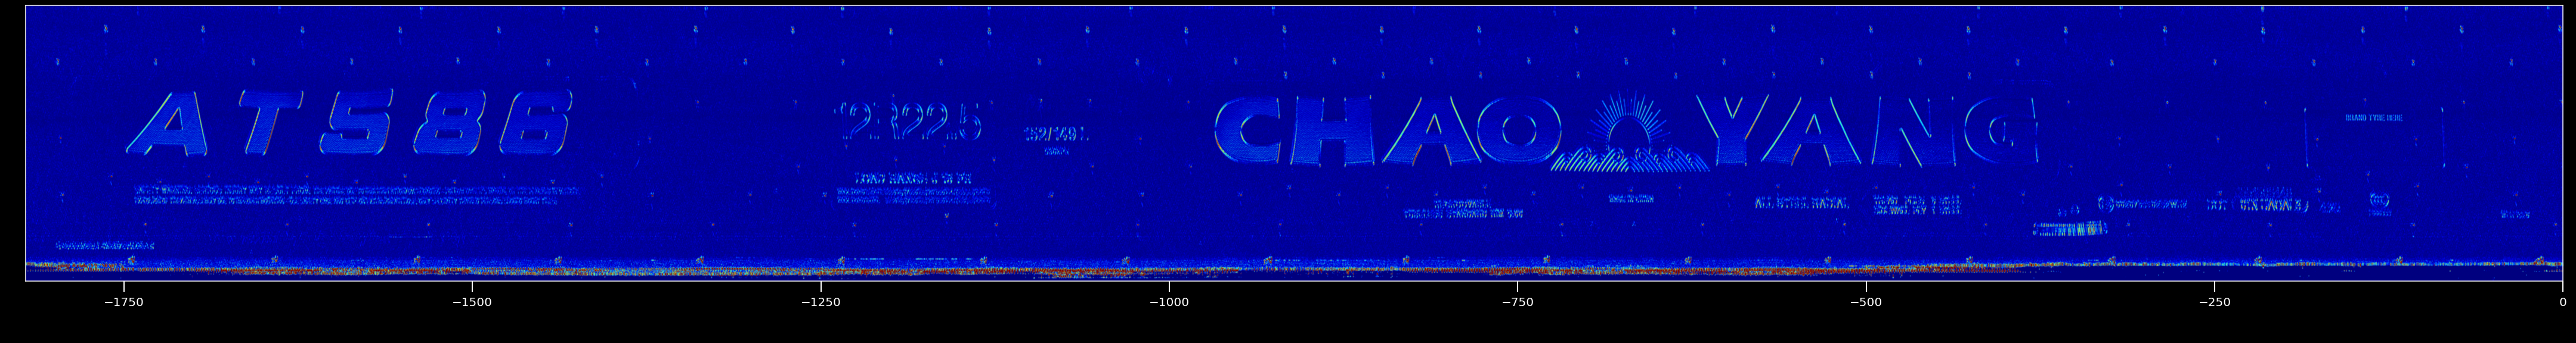
\includegraphics[width=1.0\textwidth]{figures/pointcloud_full_overview_teacher_style_smooth.png}
    \caption{全量点云改进方法得到的完整展开残差图（展示层保边增强与动态范围压缩）}
    \label{fig:full_overview}
\end{figure}

\begin{figure}[H]
    \centering
    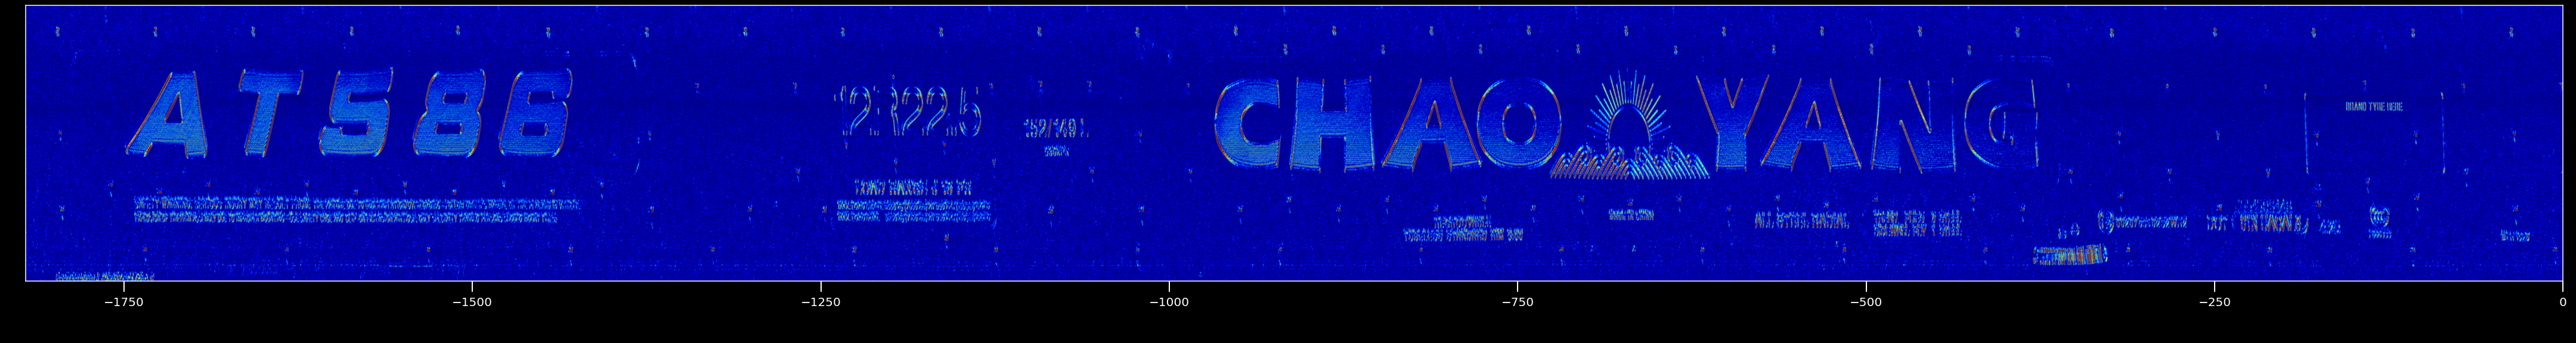
\includegraphics[width=1.0\textwidth]{figures/pointcloud_full_overview_teacher_style_detail_band.png}
    \caption{完整展开图的有效文字带放大显示}
    \label{fig:full_overview_detail_band}
\end{figure}

\subsection{Baseline 与 Improved 对比}

\autoref{fig:compare} 展示了默认局部区域 $Y\in[-200,0]$ 上 baseline 与 improved 的对比。左图中背景存在较明显的竖向纹理和块状边界，右图采用滑动窗口后，背景更加均匀，竖向块纹明显减弱，字符和局部标记仍然保留。

\begin{figure}[H]
    \centering
    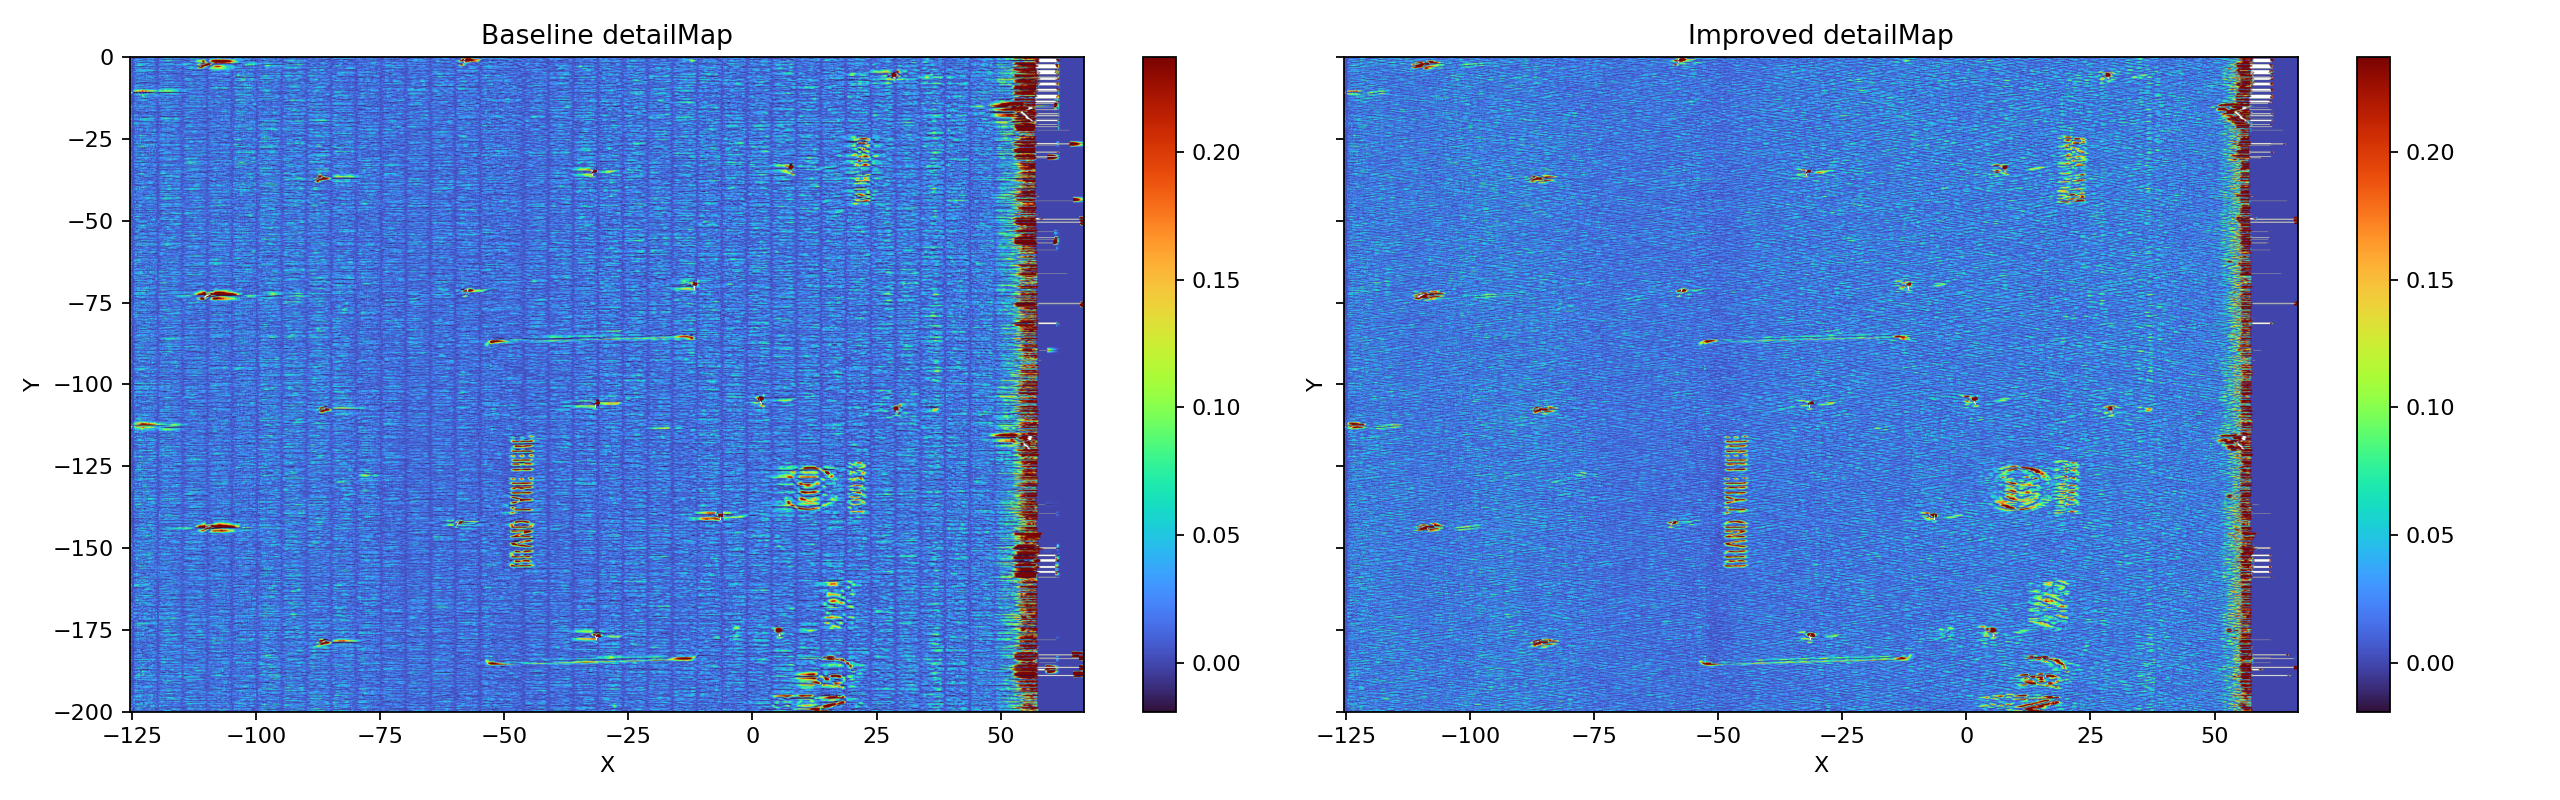
\includegraphics[width=1.0\textwidth]{figures/pointcloud_compare_baseline_improved.png}
    \caption{Baseline 与 Improved 残差图对比}
    \label{fig:compare}
\end{figure}

\subsection{剖面结果}

\autoref{fig:profile} 给出了改进方法中的样例行剖面与列剖面。行剖面中，红色总基线跟随原始高度的低频趋势，蓝色残差则突出局部突起；列剖面中，第一遍基线和第一遍残差反映了沿扫描方向的低频校正过程。

\begin{figure}[H]
    \centering
    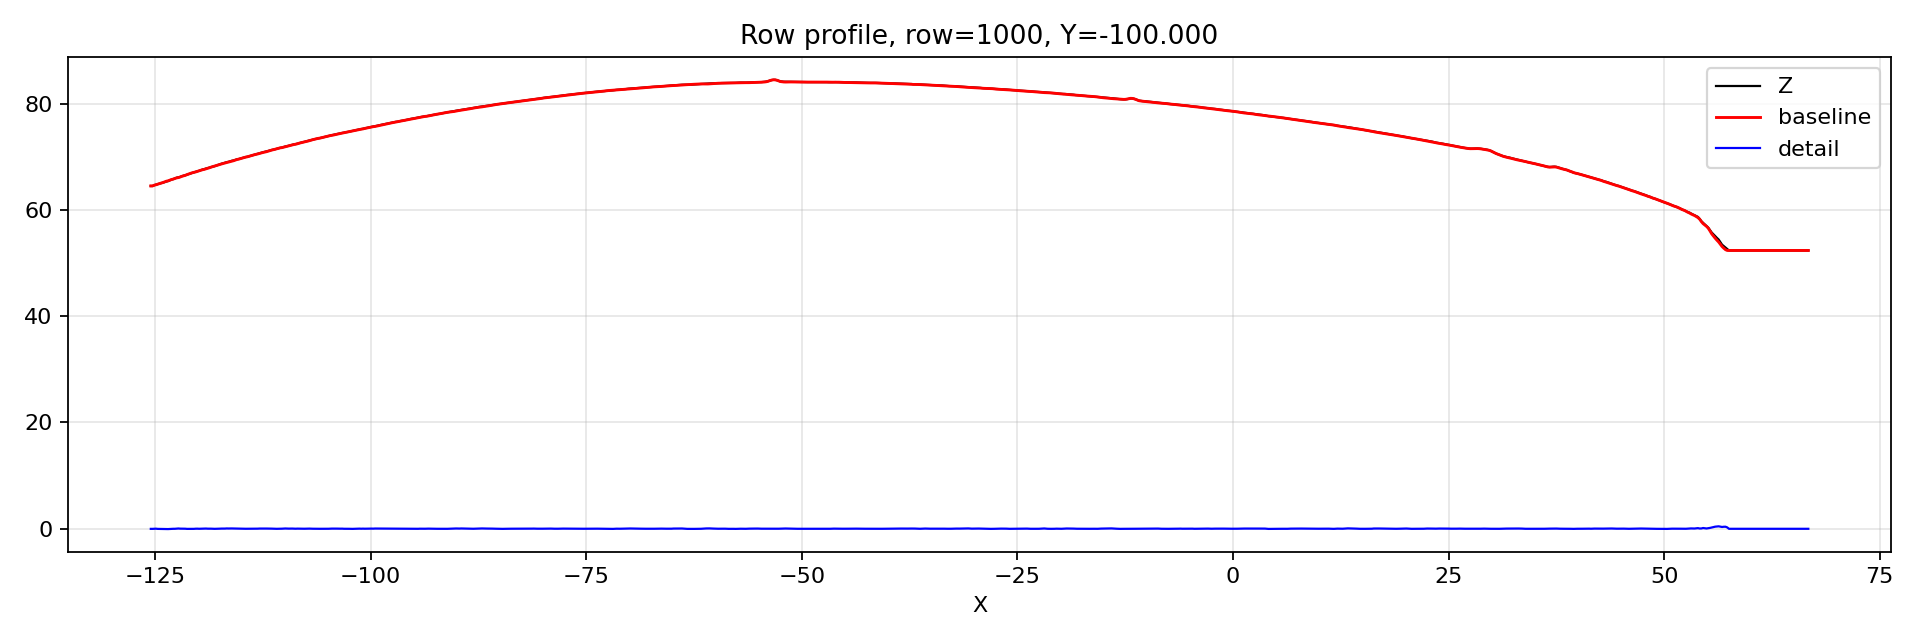
\includegraphics[width=0.48\textwidth]{figures/pointcloud_profile_row.png}
    \hspace{0.02\textwidth}
    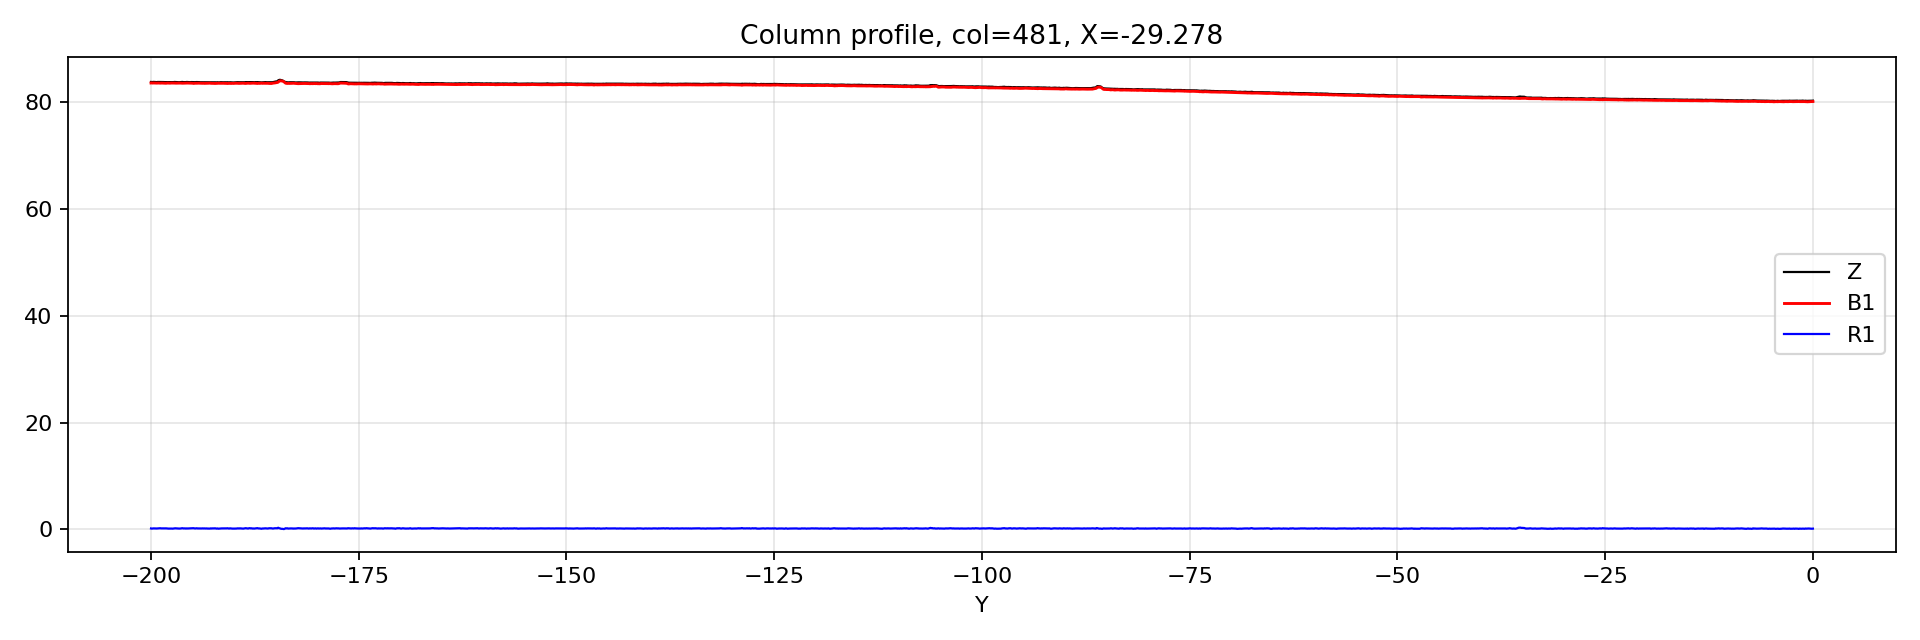
\includegraphics[width=0.48\textwidth]{figures/pointcloud_profile_col.png}
    \caption{改进方法的行剖面与列剖面}
    \label{fig:profile}
\end{figure}

\section{参数敏感性分析}

为了分析低分位值参数对结果的影响，在滑动窗口框架下分别测试了 $q=5\%$、$q=10\%$ 和 $q=15\%$。结果见\autoref{fig:q_sensitivity}。$q=5\%$ 更接近下包络，字符和局部高亮更强，但也更容易保留异常点影响；$q=15\%$ 背景更平稳，边界异常略小，但部分细节对比度下降；$q=10\%$ 在细节保留与背景平坦之间较为均衡，因此作为最终主结果。

\begin{figure}[H]
    \centering
    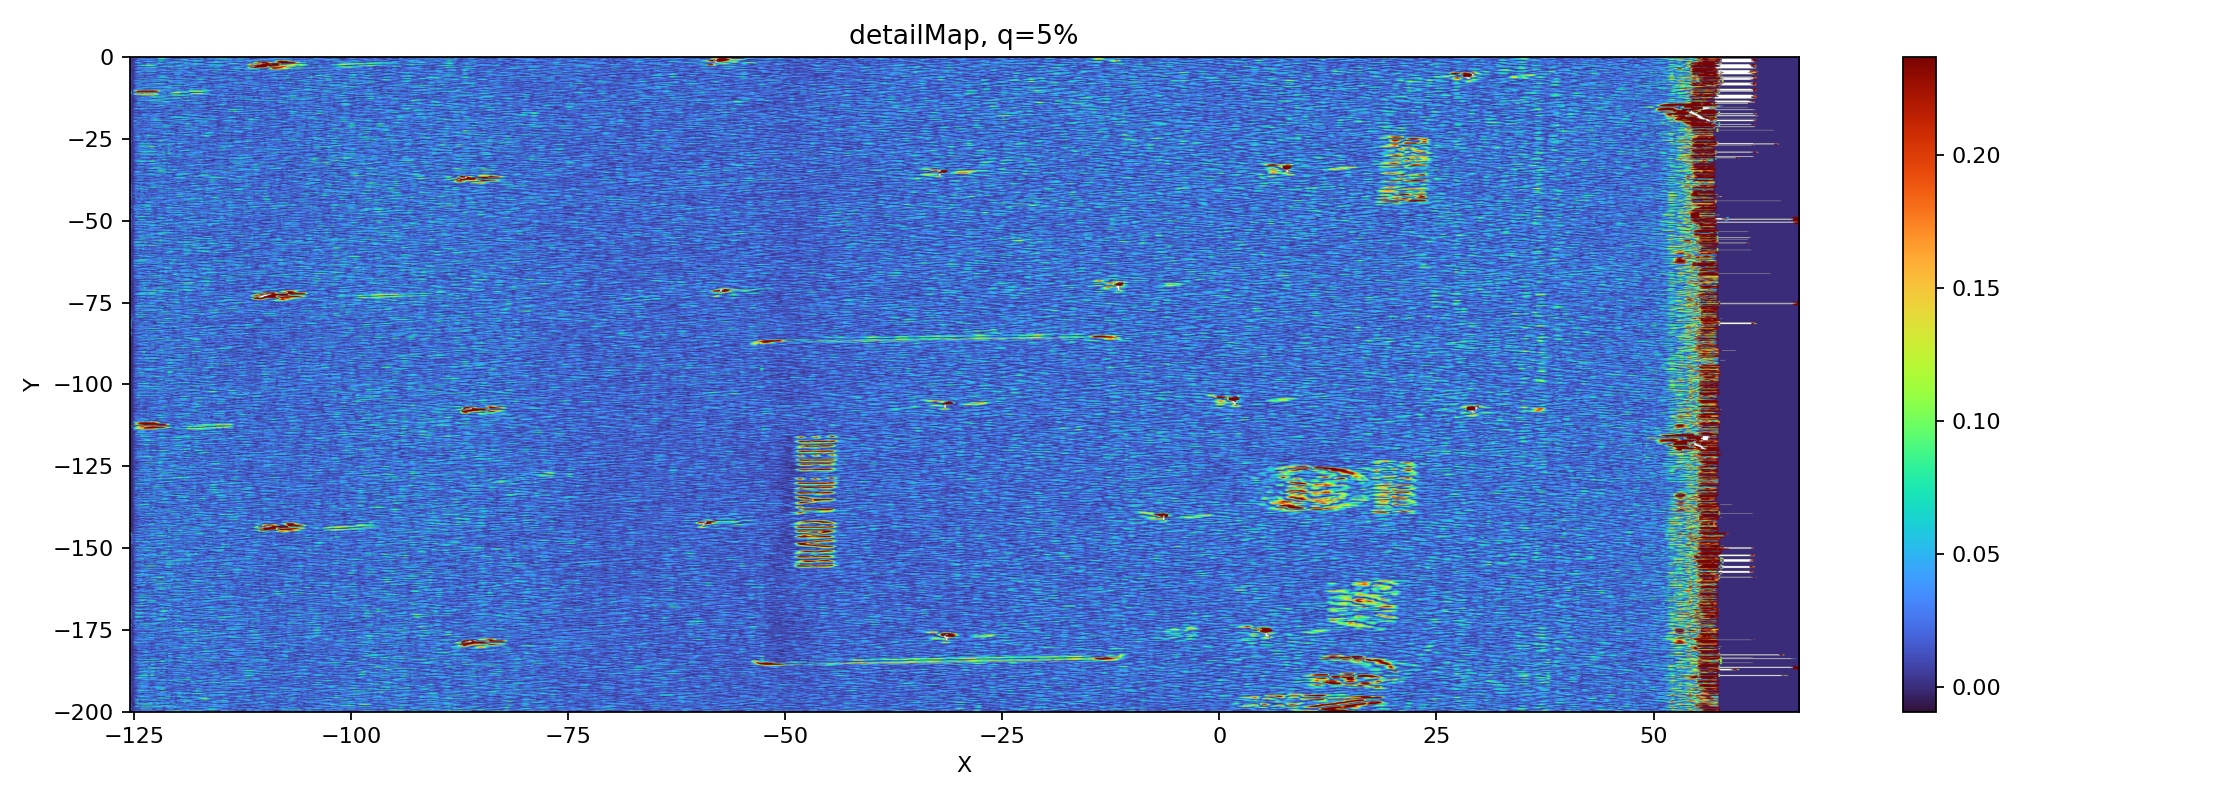
\includegraphics[width=0.32\textwidth]{figures/pointcloud_q5.png}
    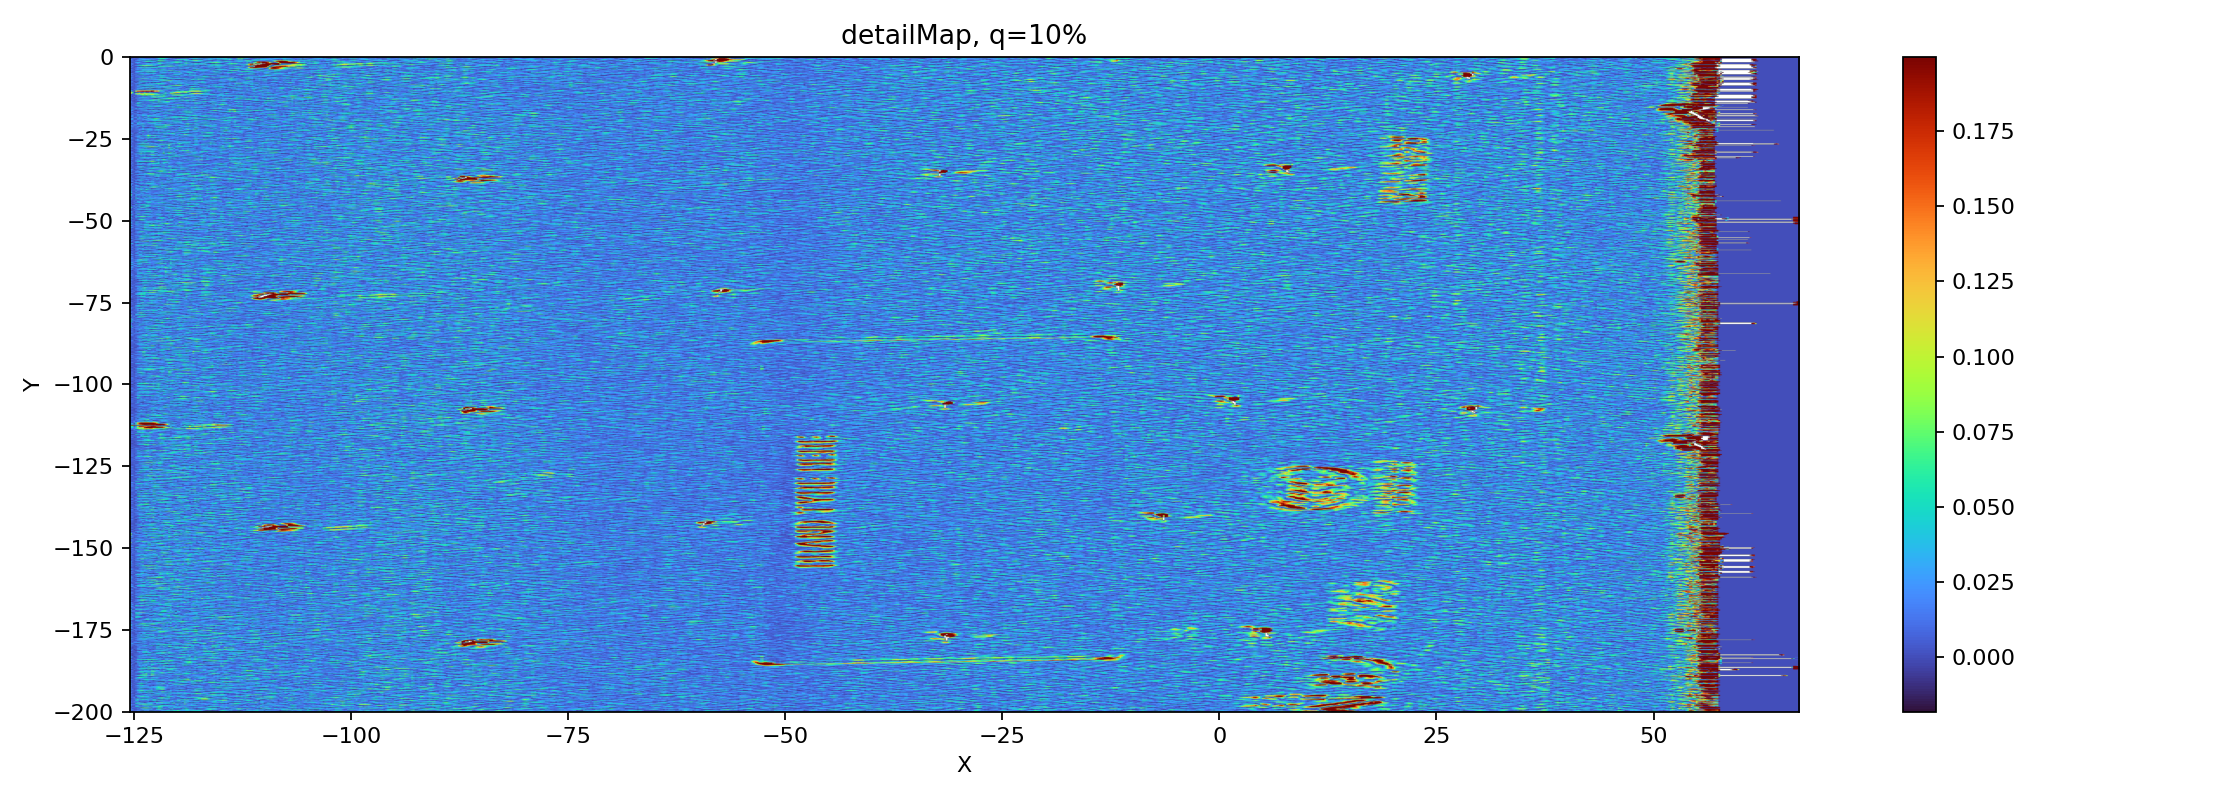
\includegraphics[width=0.32\textwidth]{figures/pointcloud_q10.png}
    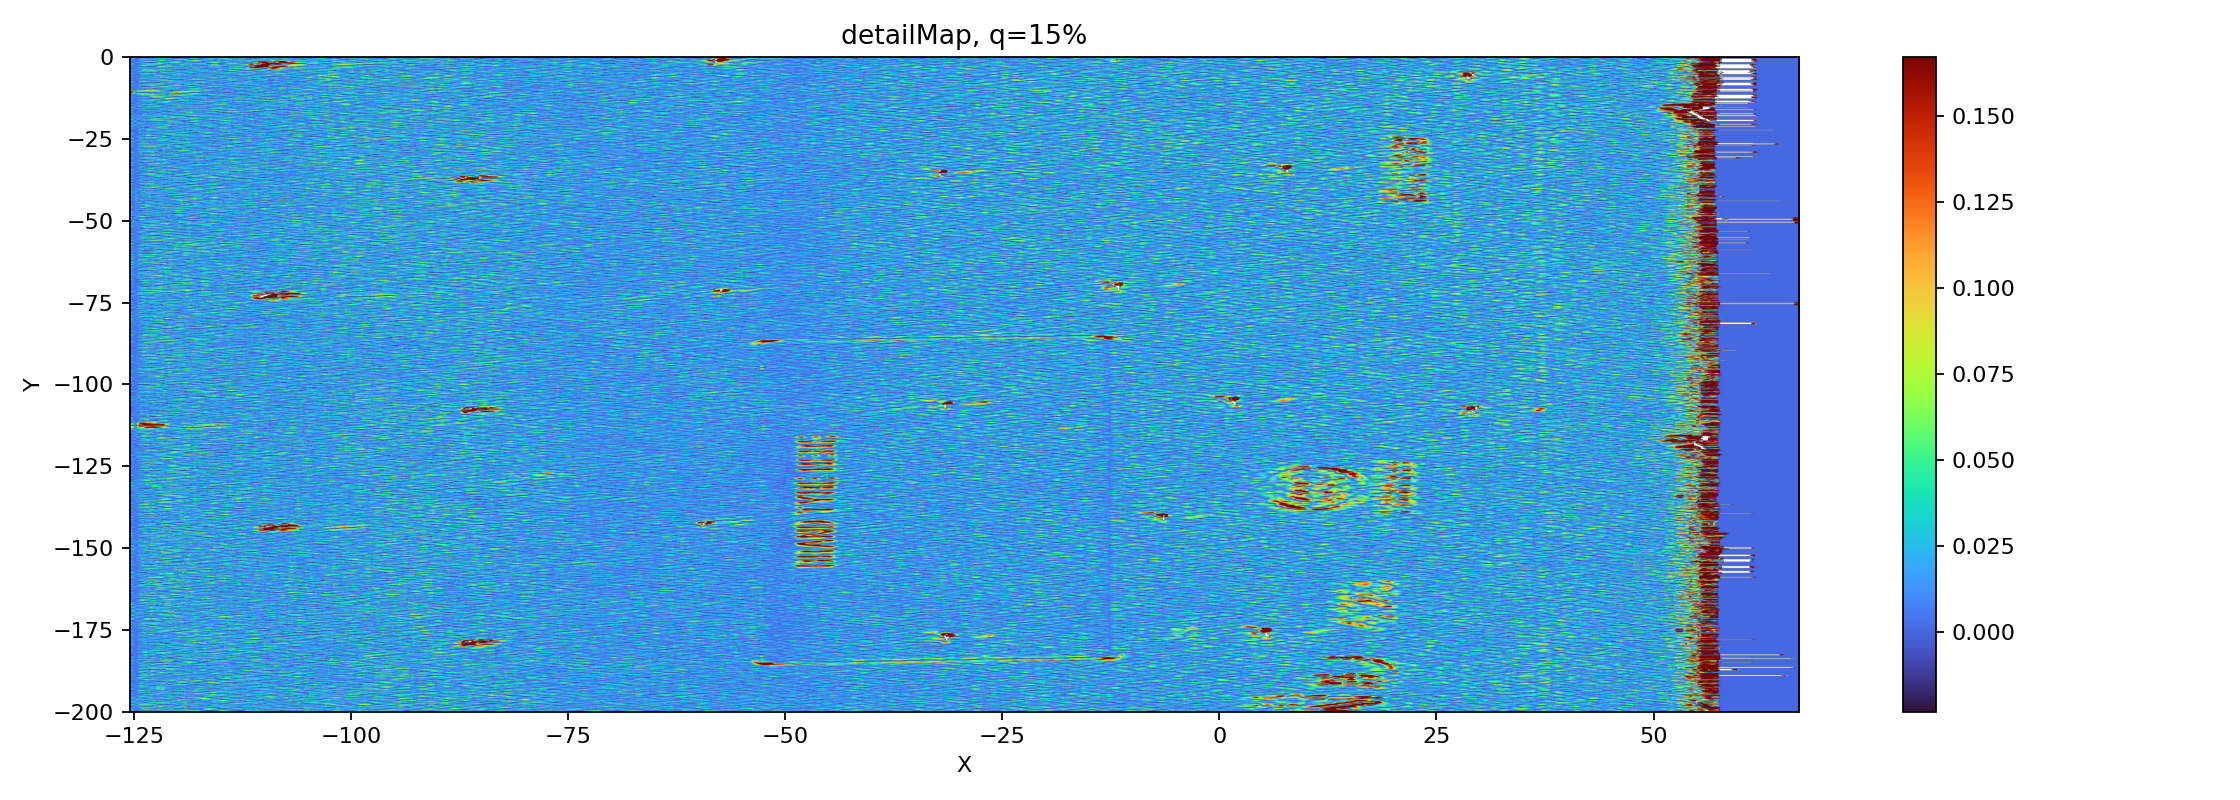
\includegraphics[width=0.32\textwidth]{figures/pointcloud_q15.png}
    \caption{滑动窗口方法中不同低分位值参数的结果对比：左为 $q=5\%$，中为 $q=10\%$，右为 $q=15\%$}
    \label{fig:q_sensitivity}
\end{figure}

\subsection{半定量指标}

由于本实验没有严格真值，评价以定性观察为主，同时辅以背景标准差、高亮对比度、边界异常强度等指标。默认局部区域的结果见\autoref{tab:metrics}。

\begin{table}[H]
    \centering
    \begin{tabular}{lccccc}
        \toprule
        方法 & 背景中位数 & 背景标准差 & 高亮对比度 & 负向凹陷 & 边界异常 \\
        \midrule
        baseline block q10 & 0.0153 & 0.0131 & 0.2567 & 0.0352 & 0.0251 \\
        improved sliding q10 & 0.0179 & 0.0141 & 0.1816 & 0.0360 & 0.0241 \\
        \bottomrule
    \end{tabular}
    \caption{Baseline 与 Improved 的半定量指标对比}
    \label{tab:metrics}
\end{table}

从指标上看，改进方法的边界异常强度略有下降，高亮对比度下降则说明部分尖锐异常被压制；结合图像观察，滑动窗口主要改善了竖向块状伪影，而不是单纯追求更高的残差峰值。该结果符合本实验目标：减少非真实结构的拖尾和网格感，同时保留可识别字符。

\section{总结与讨论}

本实验完成了点云轮廓基线估计的 Python 版本实现，并成功从 MATLAB 的 \texttt{pointCloud} 对象中解析出原始点云。通过构造规则二维高度图、两步一维基线估计和残差可视化，复现了老师给出的初始处理思路。针对初始方法中的字符局部削弱、竖向拖尾、块状纹理和边界厚化等问题，实验采用滑动窗口低分位值与控制点轻微平滑进行改进。

实验结果表明，滑动窗口方法能够显著减弱不重叠分块带来的竖向块纹，使背景更加均匀；全量展开图中，轮胎上的大字符、品牌文字、规格文字和周期性标记均能较清晰地呈现。该方法仍有局限：边界区域由于点云稀疏和轮胎几何边缘本身的影响，仍会保留较强亮带；部分细小字符在不同分位值下会出现对比度变化。后续可以尝试二维鲁棒曲面拟合、边界镜像扩展或字符候选区域保护掩膜，以进一步减少边界异常和局部误扣除。

\appendix
\renewcommand{\thesection}{\Alph{section}}

\section{项目目录与产物}

\begin{python}
exp4/
+-- code/
|   +-- baseline_estimation_python.py
|   +-- pc1.mat ... pc6.mat
|   +-- integrate1line_all2D (1).m
+-- results/
|   +-- exp4_baseline_estimation_python/
|   |   +-- 00_Zmap.png
|   |   +-- compare_baseline_vs_improved.png
|   |   +-- metrics_baseline_vs_improved.csv
|   |   +-- parameter_sensitivity/
|   +-- overview_full/
|       +-- overview_improved_detail.png
|       +-- overview_improved_detail_teacher_style.png
|       +-- overview_improved_detail_teacher_style_smooth.png
|       +-- overview_improved_detail_teacher_style_detail_band.png
+-- report/
|   +-- main.tex
|   +-- figures/
+-- README.md
\end{python}

\section{主要命令}

\begin{python}
python3 -m venv .venv
.venv/bin/python -m pip install -r requirements.txt

.venv/bin/python code/baseline_estimation_python.py

.venv/bin/python code/baseline_estimation_python.py \
    --full --overview-only --out results/overview_full
\end{python}

\end{document}
